\section{KNN}
KNN, veri noktalarının komşularına dayalı olarak sınıflandırılmasını veya tahmin edilmesini sağlayan bir algoritmadır. Temel fikir, bir veri noktasının sınıfını veya değerini belirlemek için, bu noktanın en yakın komşularının sınıfını veya değerlerini kullanmaktır.

\begin{figure}[h]
    \centering
    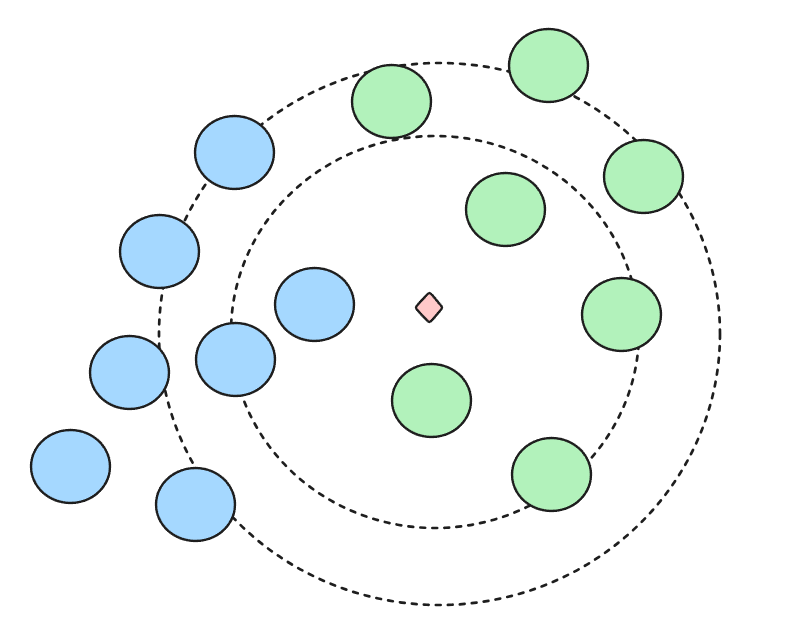
\includegraphics[width=1\textwidth]{images/knn.png}
    \caption{K-En yakın komşu.}
    \label{fig:enter-label}
\end{figure}

\subsection{Çalışma Adımları}
Tahmin yapılacak yeni veri noktası ile eğitim verilerindeki diğer noktalar arasındaki uzaklığı hesaplanır. Genellikle kullanılan uzaklık ölçüleri;
\begin{itemize}
    \item \textbf{Euclidean (Öklidyen):} İki nokta arasındaki doğru mesafeyi ölçer.
    \item \textbf{Manhattan:} İki nokta arasındaki yolların toplam uzunluğunu ölçer.
    \item \textbf{Chebyshev:} Vektörler arasındaki mutlak farkın maksimumunu alır. Daha sonra en yakın "k" komşusu seçilir. k, bir hiperparametredir ve kullanıcı tarafından belirlenmelidir.
    \item \textbf{Sınıflandırma Problemi:} Eğer KNN sınıflandırma amaçlı kullanılıyorsa, en yakın k komşunun sınıfları incelenir ve yeni veri noktasının sınıfı, bu k komşunun sınıfının çoğunluğu (modu) olarak tahmin edilir. Örneğin, eğer 3 en yakın komşu sınıfları "A", "A", ve "B" ise, yeni veri noktasının tahmini sınıfı "A" olur.
    \item \textbf{Regresyon Problemi:} Eğer KNN regresyon amaçlı kullanılıyorsa, en yakın k komşunun hedef değerleri kullanılarak yeni veri noktasının hedef değeri tahmin edilir. Genellikle bu değerlerin ortalaması veya ağırlıklı ortalaması kullanılır.
\end{itemize}

\subsection{Avantajlar}
\begin{itemize}
    \item Hızlı eğitim süresi
    \item Hem sınıflandırma hem regresyon problemlerinde kullanılabilir.
\end{itemize}

\subsection{Dezavantajlar}
\begin{itemize}
    \item Yüksek boyutlu verilerde sorun yaşayabilir çünkü uzaklık hesaplamaları artar.
    \item "k" sayısı yanlış seçilirse sonuçlar değişebilir.
    \item Eşit uzaklığa sahip birden fazla komşu olması durumunda sınıflandırma sonuçları belirsiz olabilir.
\end{itemize}

\newpage

\subsection{Hiperparametreler}
\begin{table}[h]
\centering
{\scriptsize\renewcommand{\arraystretch}{0.4}
{\resizebox*{\linewidth}{0.4\textwidth}{
\begin{tabular}{|p{3cm}|p{1cm}|p{1cm}|p{6cm}|}
\hline
Parametre & Type & Default & Açıklama \\ \hline
n\_neighbors & int & 100 & Komşu sayısını belirtir. Çok büyük k overfit'e çok küçük k underfit'e sebep olabilir. \\ \hline
weights & float & 0.1 & Komşuların etkisinin hesaplanma yöntemini belirtir. "uniform", tüm komşular eşit ağırlığa sahiptir. "distance" komşuların uzaklıklarına göre ağırlık verilir. \\ \hline
p & int & 3 & Uzaklık ölçümüü için kullanılacak metriği seçer. P=1 Manhattan uzaklık, P=2 Euclidean uzaklık olarak kullanılır. \\ \hline

\end{tabular}
}}}
\end{table}

\newpage